\title{Review of the thirteenth annual meeting}

\author{by Alexandria Wenninger\footnote{USDA Forest Service, Anchorage, Alaska, \email{alexandria.wenninger@gmail.com}}}

\maketitle

\begin{figure}[H]
\begin{center}
%\vspace{2mm}
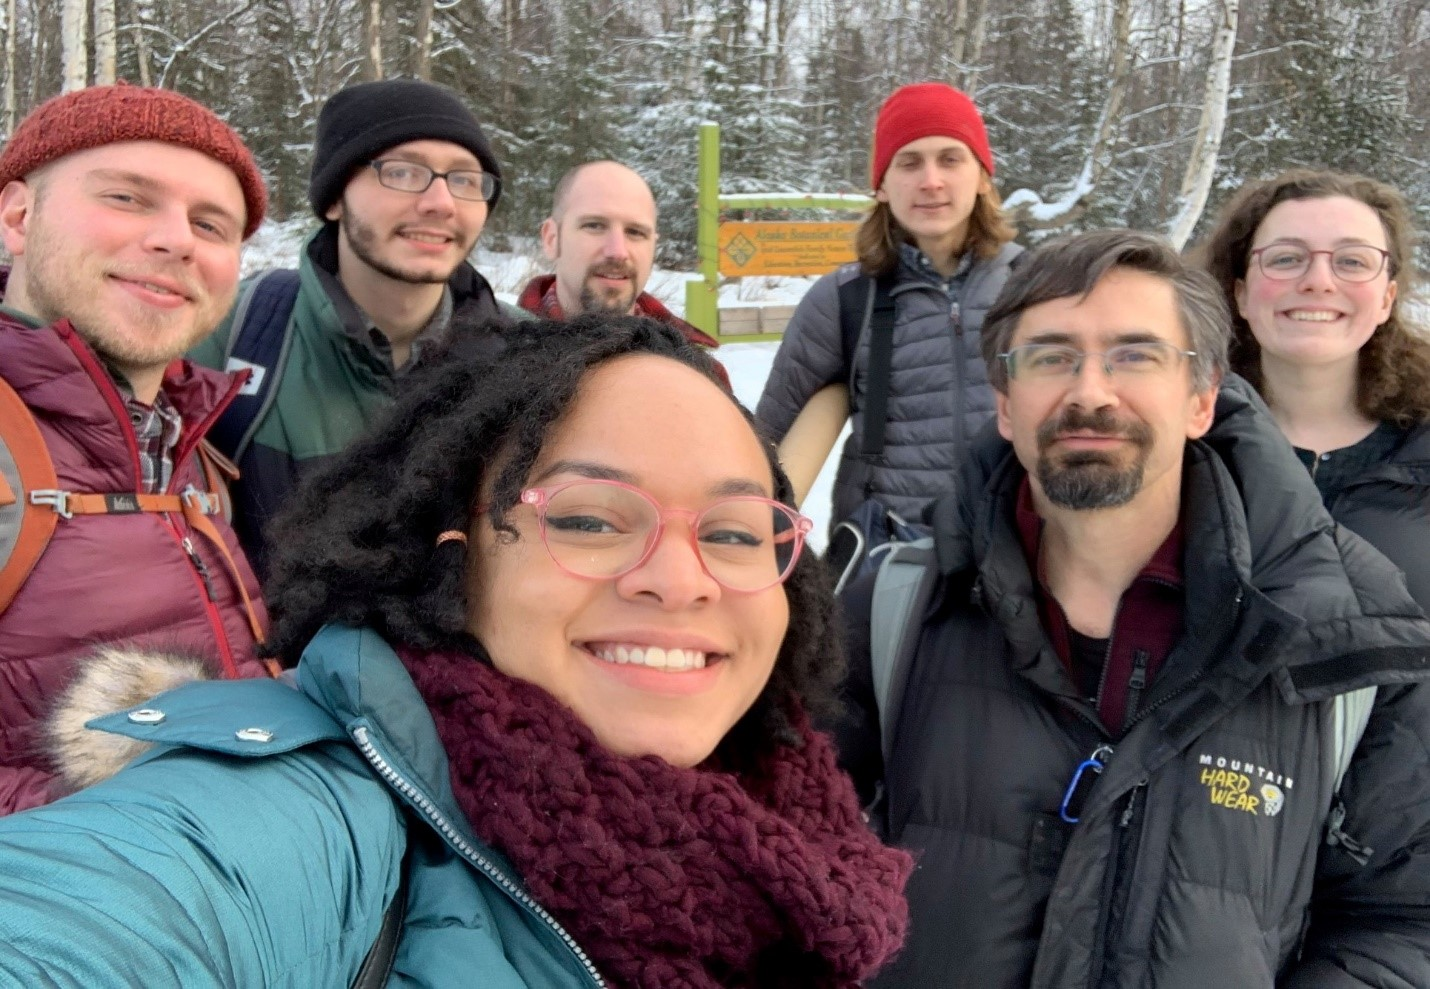
\includegraphics[width=\textwidth]{img/meeting.jpg}
\caption{\acr{UAF} crew at the 2020 \acr{AKES} meeting. Back row, left to right: Michael Apperson, Giovanni Tundo, Adam Haberski, Kyle Callegari, and Taylor Kane. Front row: Asia Sampson and Derek Sikes. Photo provided by Derek Sikes.}
\label{meeting_photo}
\end{center}
\end{figure}

The thirteenth annual meeting of the Alaska Entomological Society Meeting was held at the \href{https://www.alaskabg.org/}{Alaska Botanical Garden} greenhouse in Anchorage on February 15, 2020. We are grateful to Patrick Ryan and Stacey Shriner of the Alaska Botanical Garden for offering us the use of this space. 

\section{Presentations}

In his talk titled ``The Kenelm Philip Lepidoptera Collection no longer exists: A summary of 5 years of curdation'', \textbf{Derek Sikes} guided the audience through the process of curating lepidopterist Ken Phillip’s incredible personal collection. Most of the pinned specimens have been carefully packed and transported to the \href{https://www.si.edu/}{Smithsonian}, as per an agreement Ken had with the institute. However, as curator of the Entomology Collection at the \href{https://www.uaf.edu/museum/}{University of Alaska Museum of the North}, Derek was able to select a subset of specimens for integration into the University of Alaska Museum of the North. Ken’s hope for his incredible life work with Lepidoptera was that, one day, his collection would serve as a reference with which future lepidopteran research could compare to.

\textbf{Jessie Moan} gave an insightful view of the relationships between the public and insects through her talk, ``Fun new finds from Extension.'' As entomologist for the \href{https://www.uaf.edu/ces/}{University of Alaska’s Cooperative Extension Service}, Jessie is often the first line of contact when members of the community have questions about what insects are in their gardens, homes, and soil. Her presentation and photographs showed many exciting, interesting, and unusual insects that she has worked with recently. 
 
\textbf{Chris Fettig} returned this year to update us on his work with Spruce Beetle in Alaska. Chris is a research entomologist for the \acr{USDA} Forest Service, currently stationed at the \href{https://www.fs.fed.us/psw/}{Pacific Southwest Research Station}. He has worked extensively with bark beetles throughout North America and has interest in the indirect effects of climate change on invasive bark beetles and their forest habitats. His talk titled ``Research for new methods of control of spruce beetle (\textit{Dendroctonus rufipennis})'' gave an overview of his experiments with deterring spruce beetle attack through use of semiochemicals, and how Alaskan and Rocky Mountain populations of spruce beetle compare in their response to the same semiochemicals.

\textbf{Justin Fulkerson} and \textbf{Matt Carlson} followed with a joint presentation of the ``Seasonal pollinator diversity of rare grasslands in eastern interior Alaska.'' As botanists with the University of Alaska’s \href{https://accs.uaa.alaska.edu/}{Alaska Center for Conservation Science}, Justin and Matt have been working to understand the diversity and phenology of Alaska’s bee species. They also discussed their use of traditional barcoding as an identification aid when working with groups of bees that are difficult to identify using morphology alone.

We had several fantastic student presentations this year. This year was our first year of awarding one student for best poster presentation in addition to the student award for best oral presentation. Two posters were presented this year. \textbf{Kyle Callegari} (\acr{UAF}) presented his work, ``Interior Ecosystem: Wild, Living, Arthropod Divesity in the University of Alaska Museum.'' We congratulate \textbf{Adam Haberski} (\acr{UAF}), recipient of the 2020 \href{http://www.akentsoc.org/student-presentation-award}{Student Poster Award}, for his poster, ``\href{http://www.akentsoc.org/doc/Haberski_A_et_al_2020.pdf}{Beetle, spider, and bumblebee communities differ across an elevational gradient in Denali National Park, Alaska}.'' Adam conveyed an exceptional understanding of his study organisms and was especially impressive in his ability to answer difficult audience questions about the broader implications of his work. Congratulations, Adam!

In addition to the poster presentations, we also had three student oral presentations at the 2020 meeting. \textbf{Giovanni Tundo} (\acr{UAF}) presented ``How aspen tree height influences aspen leaf miner (\textit{Phyllocnistis populiella}) oviposition and performance.'' \textbf{Michael Apperson} (\acr{UAF}) presented ``Mosquito (Diptera: Culicidae) biomass in interior Alaska: No sign of decline 2003--2018.'' Finally, we congratulate \textbf{Asia Sampson} (\acr{UAF}), recipient of the 2020 \href{http://www.akentsoc.org/student-presentation-award}{Student Presentation Award}, for her talk, ``\href{http://www.akentsoc.org/doc/Sampson_A_2020.pdf}{A preliminary forensic entomology study in interior Alaska, \acr{USA}}.'' Asia showed an impressive depth of knowledge and enthusiasm for her work, which was especially remarkable considering all her work was done within a semester capstone project. Congratulations, Asia!


	
\section{Business items---highlights}

\begin{itemize}

\item We thank Michael Baldwin for his generous donation of a limited-edition mosquito art print made by Michael Blackstock. This item was available by auction through eBay after the meeting, starting bid \$50. 

\item Starting this year, science fair awards will consist of a physical Bioquip certificate that can be handed to the winner (either by \acr{AKES} representatives or by science fair personnel), along with a certificate of recognition from \acr{AKES} with a space for the student’s name to be written on. In previous years we have experienced significant difficulty in getting the awards to the students. These changes should streamline that process. 

\item A new long-term research project subcommittee has been created. This subcommittee will work independently of universities and government agencies. Derek Sikes, Garrett Dubois, Kyle Callegari, and Adam Haberski all volunteered to be a part of this subcommittee. 

\item Election results: Alexandria Wenninger (president), Robin Andrews (vice president), Taylor Kane (secretary), and Roger Burnside (treasurer). 

\end{itemize}

The \href{http://www.akentsoc.org/doc/AKES_meeting_20200215_minutes.pdf}{minutes} from our business meeting are available on our website.


